% *********************************************************************
% © 2021–2024 Jeremy Sylvestre
%
% Permission is granted to copy, distribute and/or modify this document
% under the terms of the GNU Free Documentation License, Version 1.3 or
% any later version published by the Free Software Foundation; with no
% Invariant Sections, no Front-Cover Texts, and no Back-Cover Texts. A
% copy of the license is included in the appendix entitled “GNU Free
% Documentation License” that appears in the output document of this
% PreTeXt source code. All trademarks™ are the registered® marks of
% their respective owners.
%
% *********************************************************************

\newcommand*{\xmin}{0}
\newcommand*{\xmax}{10}
\newcommand*{\ymin}{-30}
\newcommand*{\ymax}{45}

%
% DE is
%    dq/dt = - r * (M - q) * (T - q) * q
%  with T < M
% Here we will take r = 1, T = 4, and M = 8
% Peaks of rate function occur at
%   q = [ (M + T) ± sqrt(M² - MT + T²) ] / 3
%

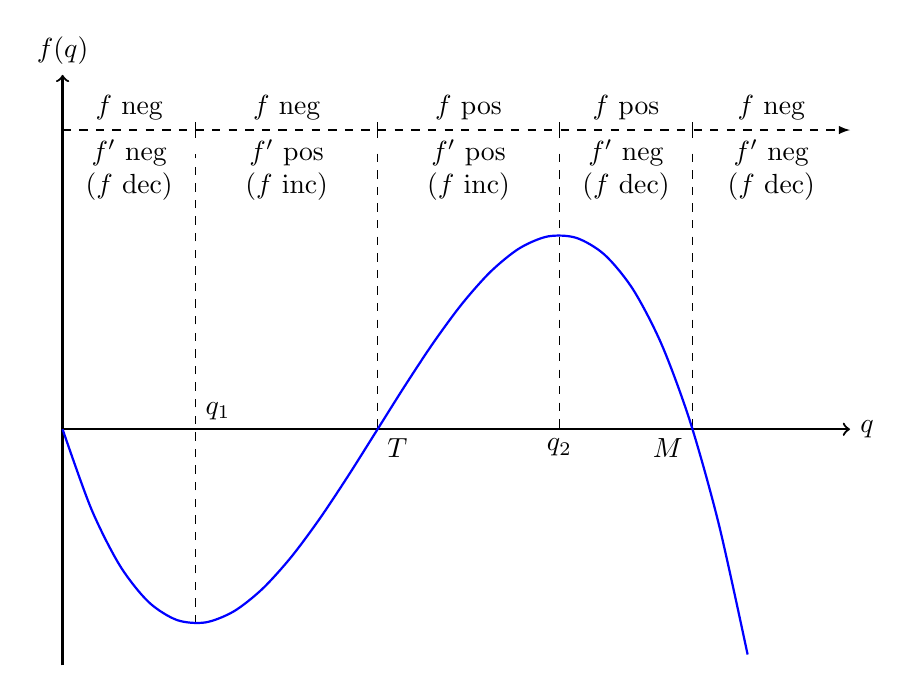
\begin{tikzpicture}
[
	closedpt/.style={circle,draw,fill,inner sep=0pt,minimum size=4pt},
	openpt/.style={circle,draw,inner sep=0pt,minimum size=4pt},
	yscale=0.1
]

	% axes
	\draw[->,thick] (0,0) -- (\xmax,0) node[right] {$q$};
	\draw[->,thick] (0,\ymin) -- (0,\ymax) node[above] {$f(q)$};

	\draw[dashed] (1.691,-24.634) -- (1.691,35);
	\node[above right] at (1.691,0) {$q_1$};
	\draw[dashed] (4,35) -- (4,0) node[below right] {$T$};
	\draw[dashed] (6.309,35) -- (6.309,0) node[below] {$q_2$};
	\draw[dashed] (8,35) -- (8,0) node[below left] {$M$};

	\draw[thick,blue,smooth,domain=0:8.7] plot (\x, { (8 - \x) * (\x - 4) * \x });

	\begin{scope}[yshift=38cm]

	\draw[dashed,-latex] (0,0) -- (\xmax,0);

	\draw (1.691,-1) -- (1.691,1);
	\node[above] at (0.845,0) {$f$ neg};
	\node[below,align=center] at (0.845,0) {$f'$ neg \\ ($f$ dec) };

	\draw (4,-1) -- (4,1);
	\node[above] at (2.846,0) {$f$ neg};
	\node[below,align=center] at (2.846,0) {$f'$ pos \\ ($f$ inc)};

	\draw (6.309,-1) -- (6.309,1);
	\node[above] at (5.155,0) {$f$ pos};
	\node[below,align=center] at (5.155,0) {$f'$ pos \\ ($f$ inc)};

	\draw (8,-1) -- (8,1);
	\node[above] at (7.155,0) {$f$ pos};
	\node[below,align=center] at (7.155,0) {$f'$ neg \\ ($f$ dec)};

	\node[above] at (9,0) {$f$ neg};
	\node[below,align=center] at (9,0) {$f'$ neg \\ ($f$ dec)};

	\end{scope}

\end{tikzpicture}
